%!TEX encoding = UTF8
%!TEX root =notes.tex

\chapter{Droites et fonctions affines}

Le but de ce chapitre est de traiter la partie fonctionnelle de la section \og Représenter et caractériser les droites du plan \fg du bulletin officiel.
Il s'agira d'étudier les équations de droite (cartésienne et réduite) ainsi que ses paramètres : son coefficient directeur (la pente) et son ordonnée à l'origine.

Les capacités attendues sont les suivantes.
	\begin{itemize}
		\item Déterminer une équation de droite à partir de deux point ou un point et la pente.
		\item Déterminer la pente d'une droite donnée par une équation ou une représentation graphique.
		\item Tracer une droite en connaissant son équation cartésienne ou réduite.
		\item Déterminer si deux droites sont parallèles ou sécantes.
		\item Résoudre un système de deux équations linéaires à deux inconnues, déterminer le point d'intersection de deux droites sécantes.
	\end{itemize}

\section{Lecture graphique et définitions}\label{sec:aff-1}

Soit $(d)$ une droite \emph{non verticale} qu'on plonge dans un repère orthonormé.
On suppose $(d)$ non verticale pour qu'elle soit la courbe représentative d'une certaine fonction $f$ qu'on souhaite déterminer : \[(d) = \C_f. \]
Posons en outre $\D = \R$ le domaine de $f$, soit la droite réelle toute entière.

On a supposé $(d)$ non verticale car dans le cas contraire, un certain antécédent $x$ aurait plusieurs images, ce qui n'est pas possible d'après la définition d'une fonction.


	\begin{center}
%	\begin{tikzpicture}[>=stealth, scale=1]
%	\begin{axis}[xmin = -4, xmax=4, ymin=-13, ymax=9, axis x line=middle, axis y line=middle, axis line style=<->, xlabel={}, ylabel={}, ticks=none, grid=both]
%		\addplot[myb, thick, domain =-3:3, samples=2] {-3*x-3}  node[above=3pt] {$(d)$};
%		\addplot[myb, thick, dotted, domain =-4:-3, samples=2] {-3*x-3} ;
%		\addplot[myb, thick, dotted, domain =3:4, samples=2] {-3*x-3};
%	\end{axis}
%	\end{tikzpicture}
	\begin{tikzpicture}[>=stealth, scale=1.2]
	\begin{axis}[xmin = -4, xmax=4, ymin=-13, ymax=9, axis x line=middle, axis y line=middle, axis line style=<->, xlabel={}, ylabel={}, ticks=none, grid=both]
		\addplot[myb, thick, domain =-3.5:3, samples=2] {-3*x-3}  node[above=3pt] {$(d)$};
		\addplot[myb, thick, dotted, domain =-4:-3.5, samples=2] {-3*x-3} ;
		\addplot[myb, thick, dotted, domain =3:4, samples=2] {-3*x-3};
		\addplot[black, mark=*, mark size = 1] (0,-3) node[left=10pt] {$(0;b)$};
		\addplot[black, thick] (0,0) node[above right] {$O$};
	\end{axis}
	\end{tikzpicture}
	\end{center}

Comme on a supposé $(d)$ non verticale, elle coupe nécessairement l'axe des ordonnées.
Posons $(0; b)$ le point d'intersection, où $b\in\R$ est un réel désormais fixé.

%On souhaite trouver la fonction $f$ telle que $(d) = \C_f$, sa courbe représentative.
On rappelle la propriété fondamentale (voir corollaire \ref{cor:prop-fond} du chapitre \ref{chap:fonc-gen}) : 
	\begin{align*}
		(x;y) \in \C_f && \iff && y = f(x).
	\end{align*}
Prenons donc un $x \in \R$ non nul, et essayons de déterminer l'ordonnée du point de $(d)$ d'abscisse $x$ afin d'obtenir $f(x)$.

	\begin{center}
	\begin{tikzpicture}[>=stealth, scale=1]
	\begin{axis}[xmin = -4, xmax=4, ymin=-13, ymax=9, axis x line=middle, axis y line=middle, axis line style=<->, xlabel={}, ylabel={}, ticks=none, grid=both]
		\addplot[myb, thick, domain =-3.5:3, samples=2] {-3*x-3}  node[above=3pt, pos=.1] {$(d)$};
		\addplot[myb, thick, dotted, domain =-4:-3.5, samples=2] {-3*x-3} ;
		\addplot[myb, thick, dotted, domain =3:4, samples=2] {-3*x-3};
		\addplot[black, mark=*, mark size = 1] (0,-3) node[left=10pt] {$(0;b)$};
		\addplot[black, thick] (0,0) node[above right] {$O$};
		
		% (x,y)
		\addplot[violet, thick, mark=|, mark size = 1] (2.5,0) node[above] {$\color{violet} x$};
		\addplot[myr, thick, mark=-, mark size = 1] (0,-10.5) node[left] {$\color{myr} y=f(x)$};
		\draw[violet, dotted, thick] (axis cs:2.5, 0) -- (axis cs:2.5, -10.5);
		\addplot[myr, dotted, thick, domain = 0:2.5, samples=2] {-10.5};
		
		\addplot[black, mark=*, mark size = 1] (2.5,-10.5) node[right] {$({\color{violet} x},{\color{myr} y})$};
		
		\addplot[black, dotted, thick, domain = 0:2.5, samples=2] {-3};
		
		% alpha
		\addplot[myg,thick,domain=.455:2/3, samples = 30] {(-3-sqrt(4-(x*3)^2))} ;
		\addplot[myg, thick] (.7,-3) node[below right] {$\alpha$};
	\end{axis}
	\end{tikzpicture}
	\hspace{3cm}
	\begin{tikzpicture}[scale=1]
		\draw[-, thick, black] (0,0) -- (3,0) node[midway, above] {$\color{violet} |x|$};
		\draw[-, thick, black] (3,0) -- (3,-3) node [midway, right] {$\color{myr} |y-b|$};
		\draw[-, thick, myb] (3,-3) -- (0,0);
		
		% angle droit
		\draw[-, black] (2.7,0)-- (2.7, -.3);
		\draw[-, black] (2.7, -.3)-- (3, -.3);
		
		% angle
		\draw [myg,thick,domain=-45:0] plot ({.5*cos(\x)}, {.5*sin(\x)})
		node[below right] {$\color{myg}\alpha$};
	\end{tikzpicture}
	\end{center}
	
	L'angle $\alpha$ comme défini ci-dessus est constant et mesure la pente de la droite.
	On se restreint au triangle rectangle dont les sommets sont $(0;b), (x ; b)$, et $(x;y)$ pour appliquer les résultats de trigonométrie du chapitre \ref{chap:pb-geom} de géométrie.

	\begin{align*}
		\tan(\alpha) = \dfrac{|y-b|}{|x|} && \iff && |y-b| = \tan(\alpha) \cdot |x|.
	\end{align*}
	Comme la valeur absolue ne fait que supprimer le signe, on en déduit que
	\begin{align*}
		y - b = \pm \tan(\alpha) \cdot x && \iff && y = \pm \tan(\alpha) \cdot x + b,
	\end{align*}
	où $\pm$ signifie ``plus ou moins'', c'est-à-dire qu'on ne connait pas \emph{a priori} le signe et que cela n'importe pas pour l'instant.
	En posant $a = \pm \tan(\alpha)$, on a trouvé la forme de la fonction $f$ telle que $(d) = \C_f$ :
		\[ f(x) = a\cdot x + b, \]
	où $a$ et $b$ sont des nombres réels déterminés entièrement par la droite $(d)$.

\dfn{Fonction affine}{
	Un \emph{fonction affine} est une fonction $f$ associant à tout réel $x\in\R$ son image
		\begin{align}
			f(x) = ax + b, \label{eq:affine}
		\end{align}
	où $a$ et $b$ sont deux paramètres : le coefficient directeur et l'ordonnée à l'origine.
	
	La courbe représentative de $f$, $\C_f$, est une droite non verticale.
}{def:affine}

\newpage

\nt{
	De la discussion ci-dessus, on en déduit des interprétations préliminaires pour les paramètres $a$ et $b$.
		\begin{itemize}
			\item Le réel $b$ est l'ordonnée du point d'intersection de la droite avec l'axe des ordonnées.
			\item Le réel $a$ est associé à la tangente de l'angle $\alpha$ que forme la droite avec l'axe des abscisses : il mesure donc la pente de la droite. En effet, le pourcentage qu'on voit écrit sur les panneaux de signalisation de descente routière est égal la tangente de l'angle de l'inclinaison vis-à-vis de l'horizontale. Par exemple, un angle de $9$° correspond à une pente de $\tan(9) \approx 15,8\%$.
		\end{itemize}
	On verra dans la suite que le signe de $a$ correspond au caractère croissant ou décroissant de la fonction affine ; et que plus $|a|$ est grand, plus la pente est raide.
}

\ex{}{
	Considérons la fonction $id$, dite \emph{identité}, donnée par
		\[ id(x) = x \qquad \text{pour tout $x \in \R$.} \]
	Cette fonction est affine, car c'est un cas spécial de la forme \ref{eq:affine} où $a=1$ et $b=0$.
	La droite $(d) = \C_{id}$ vérifie donc
		\begin{align*}
			(x;y) \in (d) && \iff && y = x.
		\end{align*}
	Un point appartient donc à $(d)$ si et seulement si sont abscisse est égale à son ordonnée.
	
	Ainsi, $(3;3) \in (d)$ et $(-\sqrt{2}; -\sqrt{2}) \in (d)$, mais $(3;4) \notin (d)$.
	La droite restreinte à $\D = [-4 ; 4]$ est donc l'ensemble des points en bleu ci-dessous.
	
		\begin{center}
		\begin{tikzpicture}[>=stealth, scale=1]
		\begin{axis}[xmin = -4, xmax=4, ymin=-4, ymax=4, axis x line=middle, axis y line=middle, axis line style=<->, xlabel={}, ylabel={}, grid=both]
		
			\addplot[myb, thick, domain =-3:3, samples=2] {x}  node[above=3pt, left] {$(d)$};
			\addplot[myb, thick, dotted, domain =-4:-3, samples=2] {x} ;
			\addplot[myb, thick, dotted, domain =3:4, samples=2] {x};
		
			
		\end{axis}
		\end{tikzpicture}
		\end{center}
}{}

\ex{}{
	Considérons la fonction $f$ donnée par
		\[ f(x) = x+6 \qquad \text{pour tout $x \in \R$.} \]
	Cette fonction est affine, car c'est un cas spécial de la forme \ref{eq:affine} où $a=1$ et $b=6$.
	La droite $(d) = \C_{f}$ vérifie donc
		\begin{align*}
			(x;y) \in (d) && \iff && y = x+6.
		\end{align*}
	Ainsi, $(3;9) \in (d)$ et $(-\sqrt{2}; -\sqrt{2}+6) \in (d)$, mais $(6;0) \notin (d)$.
	La droite est donc l'ensemble des points en bleu ci-dessous.
	
		\begin{center}
		\begin{tikzpicture}[>=stealth, scale=1]
		\begin{axis}[xmin = -4, xmax=4, ymin=2, ymax=10, axis x line=middle, axis y line=middle, axis line style=<->, xlabel={}, ylabel={}, grid=both]
		
			\addplot[myb, thick, domain =-3:3, samples=2] {x+6}  node[above=3pt, left] {$(d)$};
			\addplot[myb, thick, dotted, domain =-4:-3, samples=2] {x+6} ;
			\addplot[myb, thick, dotted, domain =3:4, samples=2] {x+6};
		
			
		\end{axis}
	\end{tikzpicture}
	\end{center}
}{ex:droite}

\ex{}{
	Considérons la fonction $f$ donnée par
		\[ f(x) = 2,2 \qquad \text{pour tout $x \in \R$.} \]
	Cette fonction est affine, car c'est un cas spécial de la forme \ref{eq:affine} où $a=0$ et $b=2,2$.
	La droite $(d) = \C_{f}$ vérifie donc
		\begin{align*}
			(x;y) \in (d) && \iff && y = 2,2.
		\end{align*}
	Ainsi, $(3;2,2) \in (d)$ et $(-\sqrt{2}; 2,2) \in (d)$, mais $(0;0) \notin (d)$.
	La droite est donc l'ensemble des points en bleu ci-dessous.
	
		\begin{center}
		\begin{tikzpicture}[>=stealth, scale=1]
		\begin{axis}[xmin = -4, xmax=4, ymin=1, ymax=4, axis x line=middle, axis y line=middle, axis line style=<->, xlabel={}, ylabel={}, grid=both]
		
			\addplot[myb, thick, domain =-3:3, samples=2] {2.2}  node[above=3pt] {$(d)$};
			\addplot[myb, thick, dotted, domain =-4:-3, samples=2] {2.2} ;
			\addplot[myb, thick, dotted, domain =3:4, samples=2] {2.2};
			
		\end{axis}
	\end{tikzpicture}
	\end{center}
}{}

\ex{}{
	Considérons la fonction $f$ donnée par
		\[ f(x) = -2x + 1 \qquad \text{pour tout $x \in \R$.} \]
	Cette fonction est affine, car c'est un cas spécial de la forme \ref{eq:affine} où $a=-2$ et $b=1$.
	La droite $(d) = \C_{f}$ vérifie donc
		\begin{align*}
			(x;y) \in (d) && \iff && y = -2x+1.
		\end{align*}
	Ainsi, $(-1;3) \in (d)$ et $(-\sqrt{2}; 2\sqrt{2}+1) \in (d)$, mais $(1;1) \notin (d)$.
	La droite est donc l'ensemble des points en bleu ci-dessous.
	
		\begin{center}
		\begin{tikzpicture}[>=stealth, scale=1]
		\begin{axis}[xmin = -4, xmax=4, ymin=-6, ymax=10, axis x line=middle, axis y line=middle, axis line style=<->, xlabel={}, ylabel={}, grid=both]
		
			\addplot[myb, thick, domain =-3:3, samples=2] {1-2*x}  node[above=5pt] {$(d)$};
			\addplot[myb, thick, dotted, domain =-4:-3, samples=2] {1-2*x} ;
			\addplot[myb, thick, dotted, domain =3:4, samples=2] {1-2*x};
			
		\end{axis}
	\end{tikzpicture}
	\end{center}
}{}

\section{Identifications des paramètres}

\ex{}{
	Pour chaque fonction affine sur $\R$ suivante, déterminer son coefficient directeur $a$ et son ordonnée à l'origine $b$.
	\begin{multicols}{2}
	\begin{enumerate}
		\item $f(x) = 2x + 1$
		\item $f(x) = 1 + 2x$
		\item $f(x) = - x$
		\item $f(x) = -42$
		\item $f(x) = 10x + 2$
		\item $f(x) = 2 + 10x$
		\item $f(x) = 1 - x$
		\item $f(x) = 0$
	\end{enumerate}
	\end{multicols}
}{}

\lem{Ordonnée à l'origine}{
	Soit $f$ une fonction affine où $a, b \in\R$ sont ses deux paramètres réels.
		\begin{align*}
			f(x) = a x + b && (x\in\R)
		\end{align*}
	Alors
		\[ f(0) = b, \]
	et donc
		\[ (0 ; b) \in \C_f. \]
}{}

\ex{}{
	On considère la droite suivante, courbe représentative $\C_f$ d'une certaine fonction affine $f$.

		\begin{center}
		\begin{tikzpicture}[>=stealth, scale=1.2]
		\begin{axis}[xmin = -4, xmax=4, ymin=-4, ymax=4, axis x line=middle, axis y line=middle, axis line style=<->, xlabel={}, ylabel={}, grid=both]
			
			% (d)
			\addplot[myb, thick, domain =-3:3, samples=2] {2-.5*x}  node[above=3pt] {$\C_f$};
			\addplot[myb, thick, dotted, domain =-4:-3, samples=2] {2-.5*x} ;
			\addplot[myb, thick, dotted, domain =3:4, samples=2] {2-.5*x};
			
			% (0,b)
			\addplot[black, mark=*, mark size = 1] (0,2) node[above right] {$(0;2)$};
		\end{axis}
		\end{tikzpicture}
		\end{center}
	
	On regarde le point de $\C_f$ d'abscisse nulle et on considère son ordonnée.
		\begin{align*}
			(0 ; 2) \in \C_f && \iff && 2 = f(0).
		\end{align*}
	Comme $f$ est affine, elle s'écrit $f(x) = ax + b$, pour certains paramètres $a,b\in\R$ réels, et donc
		\[ 2 = f(0) = a \cdot 0 + b = b. \]
	On en déduit que le paramètre $b$ vaut $2$.
}{}

\ex{}{
	Considérons une droite $(d)$ qui contient les points
		\begin{align*}
			(0;3) \in (d) && \text{ et } && (1;8) \in (d).
		\end{align*}
	On souhaite trouver la fonction affine $f$ telle que $(d)$ soit la courbe représentative de $f$.
	La propriété fondamentale \ref{cor:prop-fond} donne donc les deux équations suivantes.
		\begin{align*}
			f(0) = 3, && \text{ et } && f(1) = 8.
		\end{align*}
	Comme $f$ est affine, on sait qu'elle s'écrit $f(x) = ax+b$ pour tout $x\in\R$ et pour certains paramètres $a,b\in\R$.
	On réécrit les équations 
		\begin{align*}
			a \times 0 + b = 3 && \text{ et } && a\times1 + b = 8, \\
			b = 3 && \text{ et } && a + b = 8.
		\end{align*}
	Par suite, $b=3$, et $a= 8-b = 8-3 = 5$. Par conséquent,
		\[ f(x) = 5x + 3 \qquad \text{ pour tout } x\in\R. \]
}{}

\lem{Coefficient directeur}{
	Soit $f$ une fonction affine où $a,b \in\R$ sont ses deux paramètres réels.
		\begin{align*}
			f(x) = a x + b && (x\in\R)
		\end{align*}
	Alors, pour tout $x\in\R$ réel,
		\[ f(x+1) - f(x) = a. \]
	On interprète l'équation ainsi :
		\begin{center}
			\og lorsqu'on augmente l'abscisse $x$ de $1$, l'ordonnée $y$ augmente de $a$ \fg.
		\end{center}
}{lem:coeff-dir}

\pf{Preuve du lemme \ref{lem:coeff-dir}}{
	Pour calculer $f(x+1)$, posons la variable intermédiaire $t = x+1$.
	On a alors
		\[ f(x+1) = f(t) = a\cdot t + b = a\cdot (x+1) + b = a \cdot x + a + b. \]
	En soustrayant $f(x) = ax+b$, on trouve bien le résultat recherché.
		\begin{align*}
			f(x+1) - f(x) &= ax + a + b - (ax + b) \\ &= ax + a + b -ax -b \\ &= a
		\end{align*}
}


\ex{}{
	On considère la droite suivante, courbe représentative $\C_f$ d'une certaine fonction affine $f$.

		\begin{center}
		\begin{tikzpicture}[>=stealth, scale=1.2]
		\begin{axis}[xmin = -1, xmax=4, ymin=-4, ymax=4, axis x line=middle, axis y line=middle, axis line style=<->, xlabel={}, ylabel={}, xtick = {-4, -3, ..., 4}, ytick = {-4, -3, ..., 4}, grid=both]
			
			% (d)
			\addplot[myb, thick, domain =-0.8:2.6, samples=2] {2-2*x}  node[above=3pt] {$\C_f$};
			\addplot[myb, thick, dotted, domain =-1:-.8, samples=2] {2-2*x} ;
			\addplot[myb, thick, dotted, domain =2.6:3, samples=2] {2-2*x};
			
			% (0,b)
			\addplot[black, mark=*, mark size = 1] (0,2) node[above right] {$(0;2)$};
			
			% (1, b+a)
			\addplot[black, mark=*, mark size = 1] (1,0) node[above right] {$(1;0)$};
			
			% (2, b+2a)
			\addplot[black, mark=*, mark size = 1] (2,-2) node[above right] {$(2;-2)$};
		\end{axis}
		\end{tikzpicture}
		\end{center}
	
	On regarde deux points de $\C_f$ dont les abscisses sont espacées de $1$ et on regarde comme leur ordonnée évolue.
	Par exemple, $(1;0)$ et $(2,-2)$. 
	Le lemme \ref{lem:coeff-dir} implique que, en prenant $x=1$,
		\begin{align*}
			f(2) - f(1) = a.
		\end{align*}
	On en déduit que 
		\[ a = (-2) - (0) = -2. \]
	En effet, on a augmenté $x$ de $1$, et l'image a augmenté de $-2$ (ou diminué de $2$).
	
	Remarquons qu'on aurait pû prendre d'autres points, par exemple $(0;2)$ et $(1;0)$, ou $(2;-2)$ et $(3;-4)$.
	La différence des ordonnées vaut bien $-2$, le coefficient directeur.	
}{}


%\exe{}{
%	Donner deux points distincts appartenant à la droite suivante.
%		\[ (d) = \{ (x,y) \text{ tq. } x,y\in\R \text{ et } y = 2x-1 \}. \]
%	Représenter la droite dans un repère.
%}{}

\ex{}{
	Soient $(1;2)$ et $(4;-4)$ deux points du plan qui appartiennent à une droite $\C_f$.
	Notons $a, b \in\R$ les paramètres de la fonction affine $f$.
		\[ f(x) = ax + b \qquad \text{pour tout $x\in\R$.} \]
	On a les équivalences suivantes
		\[ (1;2) \in \C_f \qquad\iff\qquad 2 = a\times1 + b, \]
	et
		\[ (4;-4) \in \C_f \qquad\iff\qquad -4 = a\times4 + b. \]
	Ces deux égalités étant valides simultanément, on les met dans un système :
		\[ \begin{cases*} a + b = 2, \\ 4a + b = -4. \end{cases*} \]
	En l'état, il paraît difficile de trouver les valeurs de $a$ et $b$ vérifiant le système.
	Il n'est d'ailleurs pas clair qu'il existe une solution, ou qu'il n'en existe pas une infinité.
	
	Cependant, remarquons qu'en soustrayant la deuxième équation à la première, on obtient
		\begin{align*}
			(4a + b) - (a+b) &= (-4) - (2) \\
			4a+b-a-b & = -6 \\
			3a &= -6 \\
			a &= -2
		\end{align*}
	Soustraire une équation a une autre a permis de créer une nouvelle équation dans laquelle $b$ n'apparaît pas.
	On la résoud alors tranquillement pour trouver $a=-2$.
	
	On remplace ensuite la valeur de $a$ dans une des deux équations du système pour trouver $b$ : 
		\[ b=2-a = 4.\]
	On peut désormais s'assurer que $(a;b) = (-2;4)$ vérifie bien les deux équations du système simultanément.
	On conclut donc que la fonction $f$ est donnée par
		\[ f(x) = -2x + 4 \qquad \text{pour tout $x\in\R$.} \]
}{ex:systeme-affine}

%\exe{}{
%	Vérifier que les points $(1;2)$ et $(4;-4)$ appartiennent bien à la droite 
%		\[ (d) = \{ (x,y) \text{ tq. } x,y\in\R \text{ et } y = -2x+4 \}.\]
%}{}
%
%\exe{}{
%	Décrire entièrement la droite $(d)$ contenant les points $(3;-4)$ et $(-2;14)$.
%}{}
%
%\exe{}{
%	Vérifier que la fonction affine $f$ de l'exemple \ref{ex:ant-image}, en sachant que l'image de $-112$ par $f$ est $1013$, est bien donnée par $f(x) = -\frac12 x + 957$ pour tout $x\in\R$.
%
%}{}

\exe{Approfondissement}{
	Décrire l'ensemble $\C_f$ contenant les points $(0;1), (1;0),$ et $(2;1)$ où $f(x) = ax^2 + bx + c$.
	
	Grapher la parabole, par exemple en écrivant \texttt{y=x² -2x + 1} sur GeoGebra.\footnote{\href{https://www.geogebra.org/calculator}{https://www.geogebra.org/calculator}}
	
	Montrer qu'une droite ne peut pas contenir ces trois points simultanément.
}{}

%\str{
%	La stratégie de l'exemple \ref{ex:systeme-affine} peut se généraliser.
%	Considérons $(x_A, y_A)$ et $(x_B, y_B)$ deux points distincts appartenant à une droite non verticale
%		\[ (d) = \{ (x,y) \text{ tq. } x,y\in\R \text{ et } y = ax+b \},\]
%	où $a, b\in\R$ sont deux paramètres à déterminer.
%	
%	Les deux appartenances donnent les égalités suivantes, grâce à la propriété fondamentale \ref{cor:prop-fond}.
%		\[ \begin{cases} y_A = ax_A + b, \\ y_B = ax_B + b. \end{cases} \]
%	On rappelle ici que $(x_A,y_A)$ et $(x_B,y_B)$ sont des valeurs sues, et qu'il faut déterminer $a$ et $b$ en fonction de ces valeurs.
%	
%	On soustrait la deuxième équation à la première pour éliminer la variable $b$ et obtenir
%	\begin{align*}
%		y_A - y_B &= (ax_A + b) - (ax_B + b) \\
%		y_A - y_B & = a(x_A - x_B) \\
%		a & = \dfrac{y_A - y_B}{x_A - x_B},
%	\end{align*}
%	où on a pu diviser par $x_A - x_B$ car la droite est supposée non verticale et les points sont supposés distincts.
%	
%	On peut ensuite substituer pour exprimer $b$ de façon analogue mais la formule est moins facile à retenir.
%		\[ b = y_A - \dfrac{y_A - y_B}{x_A - x_B}\cdot x_A = \dfrac{x_A y_B - x_B y_A}{x_A-x_B}. \]
%}

\nt{
	Remarquons qu'on a aussi les relations suivantes, démontrables comme pour le lemme \ref{lem:coeff-dir}.
		\begin{align*}
			f(x+2) - f(x) &= 2a  &\iff &&  a &= \dfrac{f(x+2)-f(x)}2 \\
			f(x+3) - f(x) &= 3a  &\iff && a &= \dfrac{f(x+3)-f(x)}3 \\
			f\left(x+\frac12 \right) - f(x) &= \frac12 a  &\iff && a &= 2 \cdot \left(f\left(x+\frac12\right)-f(x)\right) \\
			f\left(x+\frac13 \right) - f(x) &= \frac13 a  &\iff && a &= 3 \cdot \left(f\left(x+\frac13\right)-f(x)\right)
		\end{align*}
	Plus généralement, pour n'importe quel réel $\kappa \in\R$ non nul,
		\begin{align*}
			f\left(x+\kappa \right) - f(x) = \kappa \cdot a && \iff && a = \dfrac{f(x+\kappa) - f(x)}{\kappa}.
		\end{align*}
	Si on note $x' = x+\kappa$ on a donc
		\[ a = \dfrac{f(x') - f(x)}{x' - x}. \]
	Ceci démontre la première partie du théorème \ref{thm:param-affine}.
}

\thm{Interpolation linéaire}{
	Soit $f$ une fonction affine donnée par, pour tout $x\in\R$, et pour certains paramètres $a, b\in\R$,
		\[ f(x) = ax+b. \]
	
	Si les deux points $(x_A, y_A)$ et $(x_B, y_B)$ vérifient $x_A\neq x_B$ et appartiennent à $\C_f$, alors
		\begin{align*}
			a = \dfrac{y_A - y_B}{x_A - x_B} && \text{et} && b = \dfrac{x_A y_B - x_B y_A}{x_A-x_B}. 
		\end{align*}
}{thm:param-affine}

\nt{
	%Le théorème \ref{thm:param-affine} étend le résultat du lemme \ref{lem:coeff-dir} à une différence d'abscisses qui n'est pas forcément $1$.

	Un moyen mnémotechnique pour retenir la formule de $a$ est
		\[ a = \dfrac{\text{différence des $y$}}{\text{différence des $x$}} = \dfrac{y-y'}{x-x'} = \dfrac{dy}{dx}. \]
	L'ordre des différences ($A$ moins $B$ ou $B$ moins $A$) doit être le même au numérateur et au dénominateur mais, même s'il ne l'est pas, on aura seulement commis une erreur de signe.
	Il est donc possible d'ignorer l'ordre des points et de décider du signe après grâce au caractère croissant ou décroissant de la fonction.
	
	La formule pour $b$ n'a pas a être retenue car, une fois $a$ connu, une appartenance d'un point suffit à donner une équation pour trouver $b$.
}

\ex{}{
	On considère la droite suivante, courbe représentative $\C_f$ d'une certaine fonction affine $f$.

		\begin{center}
		\begin{tikzpicture}[>=stealth, scale=1.2]
		\begin{axis}[xmin = -1.2, xmax=1, ymin=-4, ymax=4, axis x line=middle, axis y line=middle, axis line style=<->, xlabel={}, ylabel={}, xtick = {-4, -3, ..., 4}, ytick = {-4, -3, ..., 4}, grid=both]
			
			% (d)
			\addplot[myb, thick, domain =-0.55:.9, samples=2] {-1+5*x}  node[pos = .8, above=2pt] {$\C_f$};
			\addplot[myb, thick, dotted, domain =-.6:-.55, samples=2] {-1+5*x} ;
			\addplot[myb, thick, dotted, domain =.9:1, samples=2] {-1+5*x};
			
			% 2 points
			\addplot[black, mark=*, mark size = 1] (.5,1.5) node[right] {$(0,5 ; 1,5)$};
			\addplot[black, mark=*, mark size = 1] (-.5,-3.5);
			\addplot[black] (-.8,-2.7) node{$(-0,5 ; -3,5)$};
		\end{axis}
		\end{tikzpicture}
		\end{center}
		
	Le théorème \ref{thm:param-affine} affirme que
		\begin{align*}
			a = \dfrac{1,5 - (-3,5)}{0,5 - (-0,5)}  = \dfrac{5}{1} = 5. 
		\end{align*}
	On aurait aussi pû appliquer le lemme \ref{lem:coeff-dir} avec $x=-0,5$ : lorsque $x$ augmente de $1$ en passant de $-0,5$ à $+0,5$, l'ordonnée augmente de $5$ en passant de $-1,5$ à $3,5$.
}{}


%\exe{}{
%	Calculer $a$ et $b$ de l'exemple \ref{ex:systeme-affine} à l'aide des formules ci-dessus et comparer avec les valeurs obtenues.
%}{}
%
%\exe{}{
%	Décrire entièrement la droite contenant les points $(-1;-10)$ et $(1;30)$.
%}{}
%


\section{Parallélisme et intersection}

Considérons deux fonctions $f$ et $g$, affines sur $\R$.
Les courbes représentatives $\C_f$ et $\C_g$ sont deux droites du plan.
En géométrie, on distingue alors trois cas.
	\begin{enumerate}
		\item Les droites sont sécantes en un unique point $P$.
		\item Les droites sont confondues (ou égales).
		\item Les droites sont parallèles non confondues.
	\end{enumerate}
Le deuxième cas correspond à la situation où les deux fonction sont égales : c'est le cas $f=g$.
Deux fonctions affines sont égales si et seulement si leurs paramètres (coefficient directeur et ordonnée à l'origine) sont égaux.

Nous étudions d'abord algébriquement le cas $1$ de l'intesection.
Les techniques de résolution d'équations linéaires nous mèneront naturellement vers des situations pour lesquelles deux droites n'ont pas de point d'intersection : c'est troisième cas.

\ex{}{
	Considérons deux droites $\C_f$ et $\C_g$ où, pour tout $x\in\R$,
		\begin{align*}
			f(x) = 2x+3, &&
			g(x) = -4x+8.
		\end{align*}
	On souhaite trouver les points d'intersection des deux droites, c'est-à-dire décrire l'ensemble
		\[ \C_f \cap \C_g. \]
	Soit $P(x_P;y_P)$ appartenant à l'intersection $\C_f \cap \C_g$.
	On extrait deux informations distinctes afin de connaître $x_P$ et $y_P$ :
		\begin{align*}
			P \in \C_f && \text{et} && P \in \C_g
		\end{align*}
	La propriété fondamentale \ref{cor:prop-fond} nous donne donc deux équations qu'on met dans un système car elles sont valables simultanément.
		\[ \begin{cases*} y_P = 2x_P + 3, \\ y_P = -4x_P + 8. \end{cases*} \]
	Comme on a bien sûr $y_P = y_P$, on peut écrire
		\begin{align*}
			y_P &= y_P \\
			2x_P + 3 &= -4x_P + 8 \\
			6x_P &= 5 \\
			x_P &=  \dfrac56
		\end{align*}
	Et par suite $y_P = 2\cdot\dfrac56 + 3 = \dfrac{14}3$.
	
	Nous avons donc obtenu que $P\left(\dfrac56 ; \dfrac{14}3\right)$ est l'unique point qui appartient à la fois à $\C_f$ et $\C_g$, et donc l'unique point d'intersection des droites.
	Autrement dit, 
		\[ \C_f \cap \C_g = \left\{ \left(\dfrac56 ; \dfrac{14}3\right) \right\}. \]
}{}

\nt{
	On se rassurera sur le résultat trouvé en vérifiant que le point d'intersection appartient bien aux deux droites ci-dessus.
		\begin{align*}
			f(x_P) = 2x_P + 3 = 2 \cdot \dfrac56 + 3 = \dfrac{14}3 = y_P, \\
			g(x_P) = -4x_P + 8 = -4\cdot\dfrac56 + 8 = \dfrac{14}3 = y_P.
		\end{align*}
}

\exe{}{
	Considérons deux droites $\C_f$ et $\C_g$ où, pour tout $x\in\R$,
		\begin{align*}
			f(x) = 3-x , &&
			g(x) = -2x +12.
		\end{align*}
	Déterminer $\C_f \cap \C_g$, l'ensemble des points appartenant à la fois à $\C_f$ et à $\C_g$.
}{}

\exe{}{
	Considérons deux droites $(d)$ et $(d')$ données par
		\begin{align*}
			(d) &= \{ (x,y) \text{ tq. } x,y\in\R \text{ et } y = 2x+1 \}, \\
			(d') &= \{ (x,y) \text{ tq. } x,y\in\R \text{ et } y = 2x-2 \}.
		\end{align*}
	Montrer que $(d) \cap (d') = \emptyset$, l'ensemble vide.
}{}

\qs{}{
	Considérons deux droites $\C_f$ et $\C_g$ données plus généralement par	
		\begin{align*}
			f(x) = ax+b, &&
			g(x) = a'x+b',
		\end{align*}
	où $a, a', b, b' \in \R$ sont les paramètres des droites.
	
	On souhaite déterminer $P(x_P;y_P)$ appartenant à l'intersection $\C_f \cap \C_g$, ce qui se traduit par
		\[ \begin{cases*} y_P = ax_P + b, \\ y_P = a'x_P + b'. \end{cases*} \]
	et donc, en suivant le même raisonnement que précédemment,
		\begin{align*}
			ax_P + b &= a'x_P + b' \\
			(a-a')x_P &= b'-b \\
		\end{align*}
	Ici il faut faire attention car il n'est pas toujours possible de diviser par $a-a'$ pour trouver $x_P$.
	
	Quelles conditions sur $a$ et $a'$ faut-il poser pour s'assurer qu'il existe un unique point d'intersection ?
}

\exe{}{
	Considérons deux droites $(d)$ et $(d')$ données par
		\begin{align*}
			(d) &= \{ (x,y) \text{ tq. } x,y\in\R \text{ et } y = ax+b \}, \\
			(d') &= \{ (x,y) \text{ tq. } x,y\in\R \text{ et } y = a'x+b' \},
		\end{align*}
	où $a, a', b, b' \in \R$ sont les paramètres des droites.
	
	Si $a=a'$ et $b\neq b'$, montrer que $(d)\cap(d')$ est l'ensemble vide.
	
	Si $a=a'$ et $b = b'$, montrer que $(d)\cap(d') = (d) = (d')$.
}{}

\thm{}{
	Considérons deux droites $\C_f$ et $ \C_g$ avec
		\begin{align*}
			f(x)= ax+b, && \text{ et } && g(x) = a'x+b',
		\end{align*}
	où $a, a', b, b' \in \R$ sont les paramètres des droites.
	
	On distingue alors les cas suivants sur les points d'intersection entre les droites.
		\begin{enumerate}
			\item Si $a \neq a'$, les droites $\C_f$ et $\C_g$ sont sécantes en un unique point d'intersection.
			\item Sinon $a = a'$, les droites $\C_f$ et $\C_g$ sont parallèles et on distingue deux sous-cas.
				\begin{enumerate}[label=\roman*)]
					\item Si $b\neq b'$, il n'existe aucun point d'intersection ($\C_f \cap \C_g = \emptyset$).
					\item Si $b=b'$, alors $f=g$ et les droites sont confondues ($\C_f \cap \C_g = \C_f = \C_g$).
				\end{enumerate}
		\end{enumerate}
}{}

\nt{

	Soit $f$ une fonction quelconque sur $\R$.
	Alors, par définition, nous avons
		\[ \C_f = \left\{ (x ; f(x) ) \text{ où $x$ parcourt $\R$} \right\}. \]
	Cet ensemble se réécrit également de la façon suivante.
		\[ \C_f = \left\{ (x ; y ) \text{ où $x$ parcourt $\R$ et où $y = f(x)$} \right\} \]

}{}

\dfn{Équation de droite}{
	Sot $f(x) = ax+b$ une fonction affine sur $\R$. On a
		\[ \C_f = \left\{ (x ; y ) \text{ où $x$ parcourt $\R$ et où $y =ax+b$} \right\}, \]
	et nomme alors abusivement l'équation \og $y = ax+b$ \fg, l'\emph{équation de la droite $\C_f$}.
}{}


\ex{}{
	Soit $(d)$ une droite donnée par
		\[ (d) = \{ (x,y) \text{ tq. } x,y\in\R \text{ et } y = 2x+3 \}. \]
	On souhaite déterminer une droite parallèle à $(d)$ et passant par le point $(2;1)$.
	
	On s'assure au préalable qu'on ait bien deux informations distinctes, car il faut déterminer les deux paramètres de la fonction $f(x) = ax+b$ associée à la droite à trouver.
	
	Le parallélisme à $(d)$ se traduit par l'égalité des coefficients directeurs des fonctions associées :
		\[ a = 2. \]
	L'appartenance du point $(2;1)$ donne
		\[ 1 = f(1) = 2a + b, \]
	d'où $b= 1 -2a = 1-4 = -3$.
	
	En conclusion, $f(x) = 2x - 3$, et la droite recherchée est donnée par (en violet ci-dessous)
		\[ \{ (x,y) \text{ tq. } x,y\in\R \text{ et } y = 2x-3 \}. \]
		
	\begin{center}
	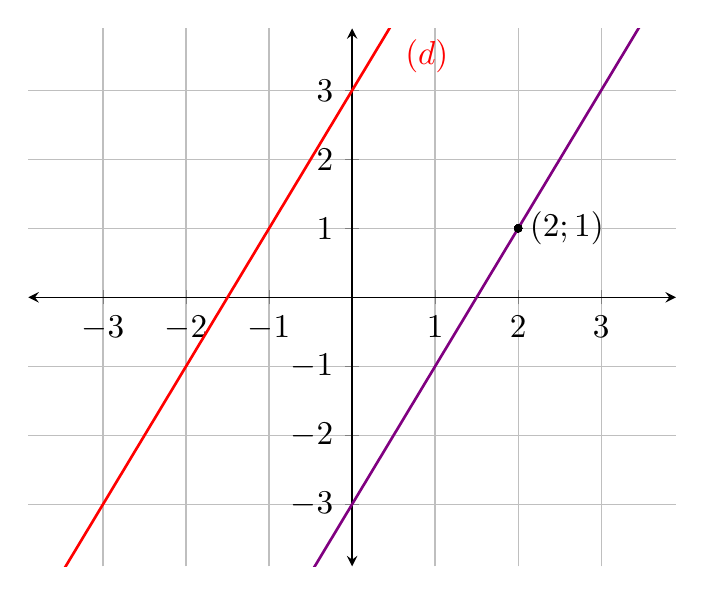
\begin{tikzpicture}[>=stealth, scale=1.2]
		\begin{axis}[xmin = -3.9, xmax=3.9, ymin=-3.9, ymax=3.9, xtick={-3,...,3}, ytick={-3,...,3}, axis x line=middle, axis y line=middle, axis line style=<->, xlabel={}, ylabel={}, grid=both]
		
			\addplot[red, thick, domain =-4:.7, samples=2] {2*x+3}  node[right=5pt, below=10pt] {$(d)$};
			\addplot[violet, thick, domain =-3:4, samples=2] {2*x-3}  node[above=3pt, left] {};
		
			\addplot[black, mark=*, mark size = 1] (2,1) node[right] {$(2;1)$};
		
		\end{axis}
	\end{tikzpicture}
	\end{center}

}{}


% postponed
%\section{Variations et signe du coefficient directeur}
%
%
%On distingue trois cas différents de droites parmis les exemples de la section \ref{sec:aff-1} : les deux premières sont croissantes, la suivante est constante, et la dernière est décroissante.
%
%\dfn{Variations}{
%	Soit $f : \D \rightarrow \R$ une fonction $f$ quelconque sur un intervalle $I\subseteq\R$.
%	Alors
%		\begin{itemize}
%			\item On dit que $f$ est \emph{croissante} si, pour tous les $x,y\in I$ du domaine,
%				\begin{align*}
%					x < y && \implies && f(x) \leq f(y).
%				\end{align*}	
%			On interprète l'implication ainsi :
%			\begin{center}
%				\og lorsqu'on augmente l'abscisse $x$, l'ordonnée $f(x)$ augmente \fg.
%			\end{center}
%				
%			\item On dit que $f$ est \emph{décroissante} si, pour tous les $x,y\in I$ du domaine,
%				\begin{align*}
%					x < y && \implies && f(x) \geq f(y).
%				\end{align*}
%			On interprète l'implication ainsi :
%			\begin{center}
%				\og lorsqu'on augmente l'abscisse $x$, l'ordonnée $f(x)$ diminue \fg.
%			\end{center}
%				
%			\item On dit que $f$ est \emph{constante} si, pour tous les $x\in I$ du domaine, et pour une certaine constante $K\in\R$,
%				\begin{align*}
%					f(x) = K.
%				\end{align*}
%		\end{itemize}
%	On définiera de la même façon \og strictement croissante \fg ~ (respectivement décroissante) en remplaçant l'inégalité large $\leq$ (resp. $\geq$) par l'inégalité stricte $<$ (resp. $>$).
%}{}
%
%\thm{Variations}{
%	Soit $f$ une fonction affine où $a, b \in\R$ sont ses deux paramètres réels.
%		\begin{align*}
%			f(x) = a x + b && (x\in\R)
%		\end{align*}
%	On distingue trois cas de figure.
%		\begin{itemize}
%			\item Si $a < 0$, alors $f$ est strictement décroissante.
%			\item Si $a=0$, alors $f$ est constante.
%			\item Si $a>0$, alors $f$ est strictement croissante.
%		\end{itemize}
%}{thm:affine-var}
%
%\pf{Démonstration du théorème \ref{thm:affine-var}}{
%	Si $a=0$, $f$ est clairement constante car
%		\begin{align*}
%			f(x) = b \qquad \text{ pour tout $x\in\R$}.
%		\end{align*}
%	
%	Sinon, on utilise les règles de manipulation des inégalités du théorème \ref{thm:ineg} vues au chapitre \ref{chap:3}.
%	
%	Si $a>0$, alors, pour tous les $x,y \in \R$ tels que $x < y$, on a
%		\begin{align*}
%			x &< y \\
%			a \cdot x &< a \cdot y \\
%			a \cdot x + b &< a \cdot y + b \\
%			f(x) &< f(y),
%		\end{align*}
%	et $f$ est donc strictement croissante.
%	
%	Si $a<0$, alors, pour tous les $x,y \in \R$ tels que $x < y$, on a
%		\begin{align*}
%			x &< y \\
%			a \cdot x &> a \cdot y \\
%			a \cdot x + b &> a \cdot y + b \\
%			f(x) &> f(y),
%		\end{align*}
%	et $f$ est donc strictement décroissante.
%}{}

